\documentclass[a4paper]{article}
\usepackage[francais]{babel}
\usepackage{graphicx}
\usepackage{wrapfig}
\usepackage[utf8]{inputenc}
\usepackage{soul}
\usepackage{scrpage2}
\usepackage{titlesec}
\usepackage{multicol}
\usepackage{tikz}
\usepackage{hyperref}
\usepackage{pbox}
\usepackage{hyperref}
\usepackage[margin=1.5cm]{geometry}
\usepackage{amsthm}
%\usepackage{multicolumn}
\usepackage{tabularx}
\usepackage[scaled]{helvet}
\usepackage{listings}
\usepackage{appendix}

\newcommand{\comment}[1]{}

\title{Rapport projet ARA 2017-2018}
\author{Mickael Rudek, Oskar Viljasaar}

\begin{document}
\maketitle


\tableofcontents

\section{Exercice 1 - Implémentation d'un MANET dans PeerSim}
\subsection{Algorithme de déplacement d'un noeud (Question 1)}

\begin{verbatim}
Movement protocol:
- if not moving
    - assign random speed lower than max
- moving
    - use `PositioningStrategiesFactory` to get next destination
    - Calc distance to next destination
    - if too far to reach `destination` in one hop
        - calculate next `x` and `y`
        - move to that position
    - if destination reached, stop
    - else continue running
\end{verbatim}
L'algorithme utilise le protocole de déplacement suivant:
Une valeur de la vitesse est aléatoirement choisie dans l'intervalle
$ \left[ \texttt{speed\_min}; \texttt{speed\_max} \right] $.
Vu qu'on est en temps discretisé, `distance\_to\_next` représente la distance parcourue au
 Une fois la destination atteinte, le noeud s'arrête pendant un tic,
 sinon il boucle en demandeant une nouvelle destination de la
 stratégie de déplacement.


 \subsection{Contenu du fichier de configuration pour la question 2}

\begin{verbatim}
simulation.endtime 50000
random.seed 5
network.size 10
init.initialisation Initialisation
control.graph GraphicalMonitor
control.graph.positionprotocol position
control.graph.time_slow 0.0002
control.graph.step 1
\end{verbatim}

\subsection{Questions 3 et 4}
Voir la sous-section 1.6.

\subsection{Implémentation de l'interface \texttt{Emitter} (Question 5)}
\begin{verbatim}
package manet.communication;

import manet.Message;
import manet.positioning.Position;
import manet.positioning.PositionProtocol;
import peersim.config.Configuration;
import peersim.core.Network;
import peersim.core.Node;
import peersim.core.Protocol;
import peersim.edsim.EDSimulator;

public class EmitterImpl implements Emitter {

    private int latency;
    private int scope;
    private int this_pid;
    private int position_protocol;

    private static final String PAR_LATENCY = "latency";
    private static final String PAR_SCOPE = "scope";
    private static final String PAR_POSITIONPROTOCOL = "positionprotocol";

    public EmitterImpl(String prefix) {
        String tmp[]=prefix.split("\\.");
        this_pid=Configuration.lookupPid(tmp[tmp.length-1]);
        this.position_protocol=Configuration.getPid(prefix+"."+PAR_POSITIONPROTOCOL);
        this.latency = Configuration.getInt(prefix + "." + PAR_LATENCY);
        this.scope = Configuration.getInt(prefix + "." + PAR_SCOPE);
    }

    @Override
    public void emit(Node host, Message msg) {
        PositionProtocol prot = (PositionProtocol) host.getProtocol(position_protocol);

        for (int i=0; i < Network.size(); i++) {
            Node n = Network.get(i);
            PositionProtocol prot2 = (PositionProtocol) n.getProtocol(position_protocol);
            double dist =prot.getCurrentPosition().distance(prot2.getCurrentPosition());
            if (dist < scope && n.getID() != host.getID()) {
                EDSimulator.add(latency, new Message(msg.getIdSrc(), n.getID(), msg.getTag(), msg.getContent(), msg.getPid()), n, msg.getPid());
            }
        }

    }

    @Override
    public int getLatency() { return latency; }

    @Override
    public int getScope() { return scope; }

    @Override
    public Object clone(){
        EmitterImpl res=null;
        try {
            res=(EmitterImpl)super.clone();
        } catch (CloneNotSupportedException e) {}
        return res;
    }
}
\end{verbatim}

\subsection{Implémentation de l'interface \texttt{NeighborProtocol} (Question 6)}


\begin{verbatim}
package manet.detection;

import manet.Message;
import manet.communication.EmitterImpl;
import peersim.config.Configuration;
import peersim.core.Node;
import peersim.edsim.EDProtocol;
import peersim.edsim.EDSimulator;

import java.util.ArrayList;
import java.util.List;

public class NeighborProtocolImpl implements NeighborProtocol, EDProtocol {
    private int this_pid;
    private int period;
    private int timer_delay;
    private int listener_pid;

    private static final String PAR_PERIOD = "period";
    private static final String PAR_TIMERDELAY = "timer_delay";
    private static final String PAR_LISTENER_PID = "listenerpid";
    Integer timeStamp = 0;

    private List<Long> neighbor_list;

    public NeighborProtocolImpl(String prefix) {
        neighbor_list = new ArrayList<>();

        String tmp[]=prefix.split("\\.");
        this_pid= Configuration.lookupPid(tmp[tmp.length-1]);
        this.period = Configuration.getInt(prefix+"."+PAR_PERIOD);
        this.timer_delay = Configuration.getInt(prefix + "." + PAR_TIMERDELAY);
        this.listener_pid = Configuration.getPid(prefix + "." + PAR_LISTENER_PID,-1);
        }

    @Override
    public List<Long> getNeighbors() { return neighbor_list; }

    @Override
    public Object clone() {
        NeighborProtocolImpl res = null;
        try {
            res = (NeighborProtocolImpl) super.clone();
            neighbor_list = new ArrayList<>();
            timeStamp = new Integer(0);
        } catch (CloneNotSupportedException e) {

        }
        return res;
    }

    @Override
    public void processEvent(Node node, int pid, Object event) {
        int emitter_pid = Configuration.lookupPid("emitter");
        EmitterImpl impl = (EmitterImpl) node.getProtocol(emitter_pid);
        Message msg = (Message) event;

        if (event instanceof Message) {
            switch (msg.getTag()) {
                case "Heartbeat":
                    if (msg.getIdSrc() == msg.getIdDest()) {
                        EDSimulator.add(this.period, event, node, pid);
                        impl.emit(node, new Message(node.getID(), 0,
                                        "Heartbeat",
                                        "Heartbeat", this_pid));
                    }
                    else {
                        if(!neighbor_list.contains(msg.getIdSrc()))
                            neighbor_list.add(msg.getIdSrc());
                        break;
                    }
                    break;
                default:
                    System.out.println("IN DEFAULT");
            }
        }
        else {
            System.out.println("no good message");
        }
        return;
    }
}
\end{verbatim}

\subsection{Influence des stratégies sur la connexité du graphe (Questions 3, 4, 8)}

\begin{itemize}
  \item Strategy1InitNext donne des positions initiales et destinations
aléatoires dans le terrain pour chaque noeud.
  \item Strategy3InitNext donne des positions initiales et
    destinations vers le milieu du terrain, dans un rayon de $ \texttt{scope} -
\texttt{marge} $, assurant un graphe
    connexe.
    \item Strategy2Next rend les noeuds immobiles, la connexité du
      graphe dépend du placement initial des noeuds.
  \item Strategy4Next assume que le graphe est connexe à
    l'initiation. Elle va déplacer un nœud dans le graphe en
    s'assurant qu'à la fin, le graphe soit toujours connexe. La
    connexité du graphe dépend du placement initial des noeuds.
    \item Strategy5Init place les noeuds en haut à droite du terrain,
      chaque noeud est placé dans le scope d'un autre noeud.
      Le graphe est initialement connexe.
      \item Strategy6Init place les noeuds en étoile au milieu du
        terrain, le graphe est donc initialement connexe.
\end{itemize}

\begin{center}
\begin{tabular}{| l | l | l |}
  \hline
  \textsl{SPI} & \textsl{SD} & \textbf{Connexe}\\
  \hline
  Strategy1InitNext & Strategy1InitNext & non\\
  \hline
  Strategy1InitNext & Strategy2Next &  non\\
  \hline
  Strategy1InitNext & \textbf{Strategy3InitNext} & \textbf{oui}\\
  \hline
  Strategy1InitNext & Strategy4Next & non \\
  \hline
  Strategy3InitNext & Strategy1InitNext & non \\
  \hline
  \textbf{Strategy3InitNext} & Strategy2Next & \textbf{oui} \\
  \hline
  Strategy3InitNext & \textbf{Strategy3InitNext} & \textbf{oui}\\
  \hline
  \textbf{Strategy3InitNext} & Strategy4Next & \textbf{oui}\\
  \hline
  Strategy5Init & Strategy1InitNext & non \\
  \hline
  \textbf{Strategy5Init} & Strategy2Next & \textbf{oui}\\
  \hline
  Strategy5Init & \textbf{Strategy3InitNext} & \textbf{oui} \\
  \hline
  \textbf{Strategy5Init} & Strategy4Next & \textbf{oui} \\
  \hline
  Strategy6Init & Strategy1InitNext & non\\
  \hline
  \textbf{Strategy6Init} & Strategy2Next & \textbf{oui} \\
  \hline
  Strategy6Init & \textbf{Strategy3InitNext} & \textbf{oui}\\
  \hline
  \textbf{Strategy6Init} & Strategy4Next & \textbf{oui}\\
  \hline
\end{tabular}
\end{center}


\pagebreak
\subsection{Impact de la portée sur la densité du graphe (Questions 10
  et 11)}

\comment{
10 itérations
\begin{center}
\begin{tabular}{|c|c|c|c|c|c|}
  \hline
Portee & SPI & SD & D & E/D & ED/D \\\hline
125 & 1 & 1 & 0.0900 +- 0.0148 & 2.0340 +- 0.2968 & 0.1940 +- 0.0220 \\\hline
250 & 1 & 1 & 0.3430 +- 0.0344 & 0.9840 +- 0.0822 & 0.1850 +- 0.0242 \\\hline
375 & 1 & 1 & 0.7130 +- 0.0447 & 0.6550 +- 0.0457 & 0.1790 +- 0.0230 \\\hline
500 & 1 & 1 & 1.1980 +- 0.0473 & 0.5700 +- 0.0460 & 0.2040 +- 0.0265 \\\hline
625 & 1 & 1 & 1.7760 +- 0.0967 & 0.4730 +- 0.0581 & 0.2120 +- 0.0366 \\\hline
750 & 1 & 1 & 2.2740 +- 0.1165 & 0.4630 +- 0.0518 & 0.2320 +- 0.0325 \\\hline
875 & 1 & 1 & 2.7320 +- 0.1012 & 0.4240 +- 0.0600 & 0.2270 +- 0.0514 \\\hline
1000 & 1 & 1 & 3.2600 +- 0.0892 & 0.4600 +- 0.0632 & 0.2740 +- 0.0541 \\\hline
125 & 3 & 3 & 2.7820 +- 0.1310 & 0.4280 +- 0.0787 & 0.2630 +- 0.0639 \\\hline
250 & 3 & 3 & 2.5410 +- 0.0575 & 0.4630 +- 0.0520 & 0.2480 +- 0.0366 \\\hline
375 & 3 & 3 & 2.3370 +- 0.1246 & 0.4380 +- 0.0371 & 0.2200 +- 0.0241 \\\hline
500 & 3 & 3 & 2.3830 +- 0.0684 & 0.4320 +- 0.0426 & 0.2300 +- 0.0335 \\\hline
625 & 3 & 3 & 2.3250 +- 0.0745 & 0.4730 +- 0.0473 & 0.2450 +- 0.0472 \\\hline
750 & 3 & 3 & 2.3170 +- 0.0714 & 0.4590 +- 0.0532 & 0.2330 +- 0.0484 \\\hline
875 & 3 & 3 & 2.3390 +- 0.1023 & 0.4400 +- 0.0369 & 0.2140 +- 0.0201 \\\hline
1000 & 3 & 3 & 2.3450 +- 0.1551 & 0.4720 +- 0.0654 & 0.2480 +- 0.0531 \\\hline
\end{tabular}
\end{center}
}

\begin{center}
\begin{tabular}{|c|c|c|c|c|c|}
  \hline
Portee & SPI & SD & D & E/D & ED/D \\\hline
125 & 1 & 1 & 0.0953 +- 0.0155 & 1.9218 +- 0.2210 & 0.1943 +- 0.0241 \\\hline
250 & 1 & 1 & 0.3441 +- 0.0302 & 0.9882 +- 0.0791 & 0.1949 +- 0.0296 \\\hline
375 & 1 & 1 & 0.7277 +- 0.0490 & 0.6890 +- 0.0724 & 0.1982 +- 0.0409 \\\hline
500 & 1 & 1 & 1.1966 +- 0.0595 & 0.5586 +- 0.0468 & 0.2049 +- 0.0278 \\\hline
625 & 1 & 1 & 1.7340 +- 0.0904 & 0.4903 +- 0.0584 & 0.2188 +- 0.0418 \\\hline
750 & 1 & 1 & 2.2763 +- 0.0774 & 0.4570 +- 0.0616 & 0.2306 +- 0.0435 \\\hline
875 & 1 & 1 & 2.7883 +- 0.0979 & 0.4585 +- 0.0743 & 0.2551 +- 0.0641 \\\hline
1000 & 1 & 1 & 3.2539 +- 0.0870 & 0.4583 +- 0.0753 & 0.2760 +- 0.0793 \\\hline
125 & 3 & 3 & 2.8025 +- 0.1088 & 0.4299 +- 0.0680 & 0.2435 +- 0.0559 \\\hline
250 & 3 & 3 & 2.4760 +- 0.0980 & 0.4381 +- 0.0446 & 0.2293 +- 0.0342 \\\hline
375 & 3 & 3 & 2.3910 +- 0.1285 & 0.4527 +- 0.0567 & 0.2355 +- 0.0429 \\\hline
500 & 3 & 3 & 2.3528 +- 0.0868 & 0.4443 +- 0.0459 & 0.2220 +- 0.0379 \\\hline
625 & 3 & 3 & 2.3267 +- 0.1107 & 0.4584 +- 0.0600 & 0.2376 +- 0.0425 \\\hline
750 & 3 & 3 & 2.3350 +- 0.1005 & 0.4686 +- 0.0626 & 0.2413 +- 0.0490 \\\hline
875 & 3 & 3 & 2.3451 +- 0.0853 & 0.4703 +- 0.0600 & 0.2500 +- 0.0516 \\\hline
1000 & 3 & 3 & 2.3639 +- 0.0991 & 0.4614 +- 0.0698 & 0.2379 +- 0.0506 \\\hline
\end{tabular}
\end{center}
Dans la stratégie 1, l'étendue de la portée a un impact sur la
connexité du graphe, la stratégie de déplacement étant celle de
choisir des destinations aléatoires dans le terrain. Il est plus
facile donc de faire un graphe connexe en prenant une valeur assez
grande pour la portée.

La stratégie 3 donnant un graphe connexe dès
le début, les noeuds disposent déjà d'un nombre de voisins important.
Augmenter la portée pour la stratégie 3 a tendance à légèrement faire
diminuer la densité du graphe. Cela peut être expliqué par la distance
aléatoire pour la prochaine destination, tirée entre
\texttt{NextDestinationStrategy.minimum\_distance} et $scope - marge$, sachant
que $marge$ est plutôt petit (20) et reste constant, alors que la
portée peut varier jusqu'à 1000. Le graphe, dans la stratégie 3, est beaucoup
plus étendu, et les noeuds peuvent avoir moins d'arcs directs
entre eux.
\begin{center}
\begin{minipage}[c]{\linewidth}
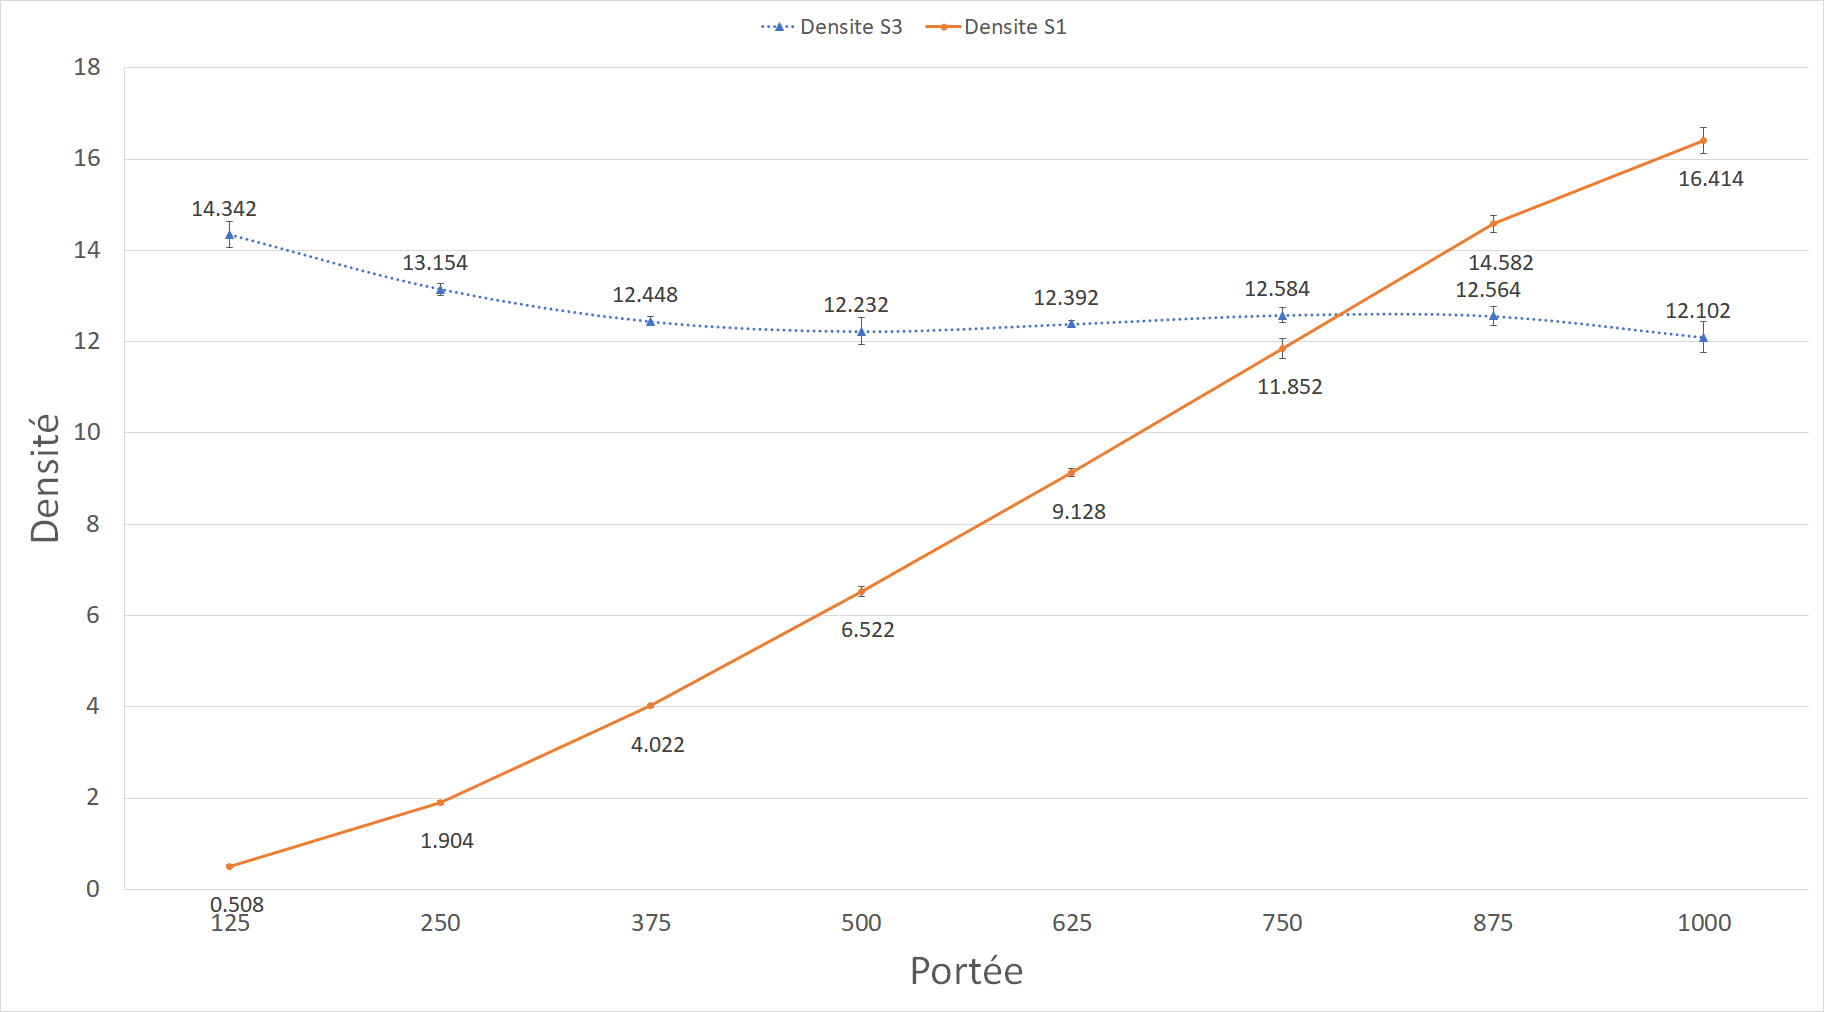
\includegraphics[width=\textwidth]{images/q10-11-s1and2.png}
\begin{center}
  Impact de la portée sur la densité avec la stratégie 1
  (orange) et la 3 (bleu).
  \end{center}
\end{minipage}
\end{center}

\section{Exercice 2}
\subsection{Question 1}
\begin{center}
\begin{tabular}{|l|r|r|}
  \hline
Taille & D-end & ED/D end \\ \hline
10 & 4.7300 +- 0.0000 & 0.9000 +- 0.0000 \\ \hline
20 & 3.8680 +- 0.9007 & 0.6580 +- 0.2134 \\ \hline
30 & 3.9380 +- 0.5319 & 0.6940 +- 0.1995 \\ \hline
40 & 3.6680 +- 0.7796 & 0.5200 +- 0.2904 \\ \hline
50 & 4.5080 +- 1.1221 & 0.9380 +- 0.4756 \\ \hline
60 & 4.0560 +- 1.0740 & 0.5080 +- 0.2393 \\ \hline
70 & 3.9260 +- 0.5985 & 0.8520 +- 0.2531 \\ \hline
80 & 3.8720 +- 0.7195 & 0.6260 +- 0.2407 \\ \hline
90 & 4.5860 +- 0.6865 & 0.7240 +- 0.2003 \\ \hline
100 & 4.1340 +- 0.2911 & 0.7020 +- 0.1132 \\ \hline
120 & 4.1900 +- 0.5124 & 0.7740 +- 0.1500 \\ \hline
140 & 4.4380 +- 1.0513 & 0.8580 +- 0.2485 \\ \hline
160 & 3.9820 +- 0.6756 & 0.6860 +- 0.2604 \\ \hline
180 & 4.2860 +- 0.5810 & 0.7640 +- 0.2772 \\ \hline
200 & 3.4300 +- 0.5758 & 0.5040 +- 0.1252 \\ \hline
\end{tabular}
\end{center}

\begin{center}
\begin{minipage}[c]{\linewidth}
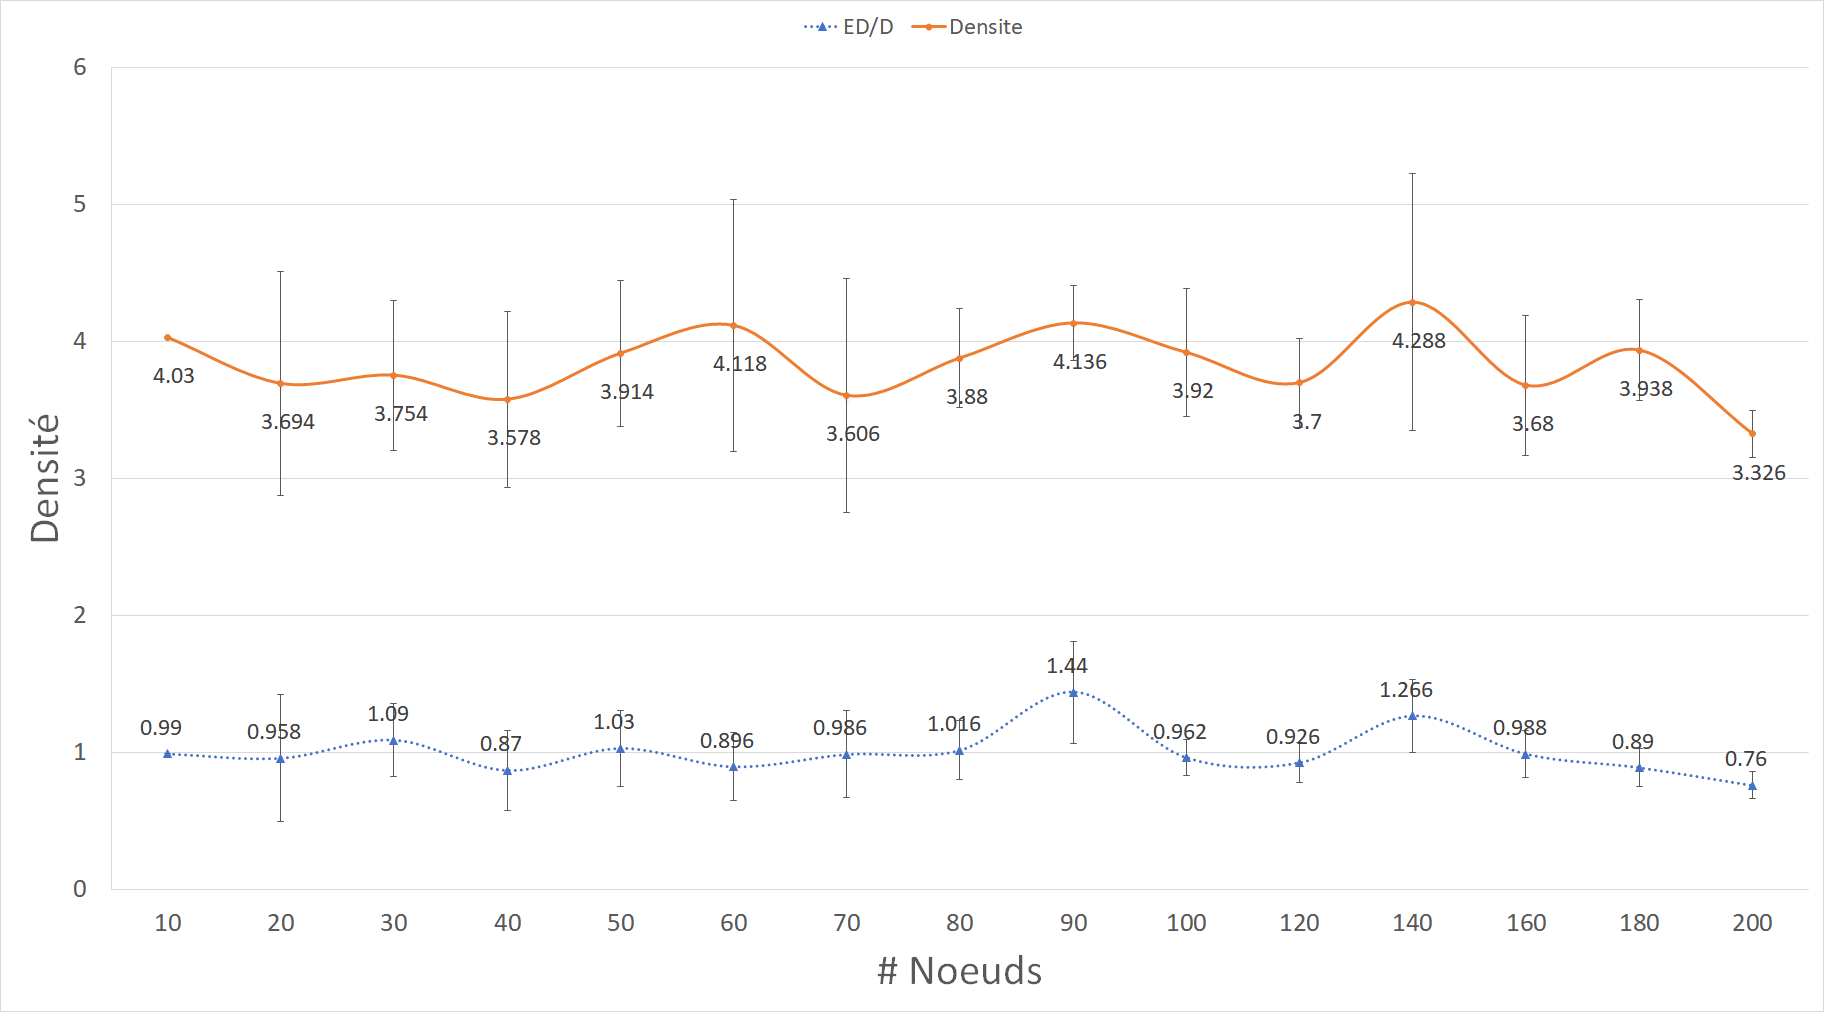
\includegraphics[width=\textwidth]{images/ex2.png}
\begin{center}
  Impact de la portée sur la densité avec la stratégie 1
  (orange) et la 3 (bleu).
  \end{center}
\end{minipage}
\end{center}


\pagebreak
\begin{appendix}
  \section{Compilation, lancement du code et jeux de test}
  \subsection{\texttt{src/Makefile}}
    Un fichier \texttt{Makefile} est inclus dans le dossier
    \texttt{src}. Celui-ci reconnaît les directives:
    \begin{itemize}
    \item \texttt{make} compile le projet.
    \item \texttt{make run} lance une instance de simulation telle que
      spécifiée dans \texttt{src/manet/cfg\_initial.txt}.
    \item \texttt{make clean} nettoie le projet des compilés.
    \item \texttt{make bench\_clean} nettoie le dossier \texttt{src}
      des dossiers de résultats des benchmarks.\\
    \end{itemize}

    Le \texttt{Makefile} admet par ailleurs deux variables:
    \begin{itemize}
    \item \texttt{DIR\_PEERSIM=<chemin>}: le dossier d'installation de
      Peersim, qu'il faudra \textbf{obligatoirement} soit modifier,
      soit spécifier dans \texttt{make} et \texttt{make run}.
    \item \texttt{CFG=<chemin>}: le chemin d'un fichier de
      configuration Peersim, initialisé à \texttt{src/manet/cfg\_initial.txt} par défaut.
    \end{itemize}

    \subsection{\texttt{src/bench.pl}}
    Exemple: \texttt{./bench.pl <chemin\_peersim>}

    Le script crée un dossier \texttt{bench\_<date>} où seront stockés les
    résultats pour la question 8 de l'exercise 1. Le dossier contiendra
    les fichiers de configuration pour les expériences sous le nom
    \texttt{cfg\_bench\_<scope>\_<SPI>\_<SD>}, les résultats d'autres
    fichiers, de même nom avec l'extension \texttt{.result}. Ces derniers contiennent les résultats de 10 expériences avec autant de différentes graines aléatoires.

    \subsection{\texttt{src/bench.py}}
    exemple: \texttt{bench.py <chemin\_results>}

    Dans le dossier \texttt{<chemin\_results>} doivent se trouver les fichiers résultats créés par \texttt{bench.pl}. Utilisé pour les resultats de benchmark, pour remplir les tableaux.

Exemple de sortie:
\begin{verbatim}
/ara/src/results/cfg_bench_500_3_3.result
| 2.3830 +- 0.0684 | 0.4320 +- 0.0426 | 0.2300 +- 0.0335 |

/ara/src/results/cfg_bench_875_3_3.result
| 2.3390 +- 0.1023 | 0.4400 +- 0.0369 | 0.2140 +- 0.0201 |

/ara/src/results/cfg_bench_750_1_1.result
| 2.2740 +- 0.1165 | 0.4630 +- 0.0518 | 0.2320 +- 0.0325 |

/ara/src/results/cfg_bench_375_1_1.result
| 0.7130 +- 0.0447 | 0.6550 +- 0.0457 | 0.1790 +- 0.0230 |
\end{verbatim}
Les valeurs correspondent à des moyennes avec écarts-type, obtenus sur
10 itérations sur chaque combinaison de SPI et SD.

\end{appendix}



\end{document}
